% introduction au cours de C++

\subsection{Pourquoi C++ dans l'option RV ?}

\begin{frame}{Qu'est-ce que C++ ?}
\begin{figure}[htbp]
\begin{center}
   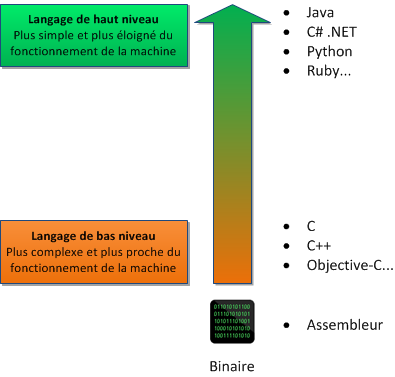
\includegraphics[scale=0.6]{fig/langages.png}
   \caption{(c) OpenClassrooms}
\end{center}
\end{figure}
\end{frame}

\subsection{Historique}

\begin{frame}{Histoire}
\begin{itemize}
\item 1958 : Algol
\item années 60 : CPL, puis BPCL puis B
\item 1970 : langage C (Dennis Ritchie 1969-1973)
\item 1979 : \textit{C with classes}
\item 1983 : C++ (amélioration du C ) : Bjarne Stroustrup
\item 1989 : C++ 2.0 (héritage multiple, classes abstraites)
\item 1995 : java
\item 1998 : début de la normalisation de C++ (inclusion de la \textit{SL})
\item 2011 : \textbf{C++11 devient un standard ISO}
\item 2014 : nouvelle norme C++14
\item 2017 : c++17 : définition figée en avril 2017, acceptation ISO/ANSI
\item 2020 : c++20 : en retard
\end{itemize}
\end{frame}

\begin{frame}[fragile]
   \frametitle{C à l'ancienne}
   \begin{itemize}
      \item Pour mémoire, C est un langage qui permet des choses un peu \emph{roots}
   \end{itemize}
   \pause 
   \begin{lstlisting}
      int a;
      a = a+++++a; // forbidden since C89
   \end{lstlisting}
   \pause
   \begin{lstlisting}
      switch(0)
      i++;
   \end{lstlisting}
   \pause 
   \begin{lstlisting}
      #define boo() 123
      #define foo(y) boo y )
      #define open (
      foo(open)
   \end{lstlisting}
   \pause
   \begin{lstlisting}
      #include<stdio.h>
      int main(){int a=0,b=a;long long c[178819],d=8,e=257,f,g,
      h,i=d-9;for(;a<178819;){c[a++]=i;}for(a*=53;a;a>>=8)putc\
      har(a);if((f=getchar())<0)return 0;for(;(g=getchar())>=0;
      ){h=i=g<<8^f;g+=f<<8;a=e<(512<<a%8|(a<7))||f>256?a:a>6?15
      :a+1;for(;c[i]>-1&&c[i]>>16!=g;)i+=i+h<69000?h+1:h-69000;
      h=c[i]<0;b|=h*f<<d;for(d+=h*(a%8+9);d>15;d-=8)putchar(b=b
      >>8);f=h?g-f*256:c[i]%65536L;if(a<8*h){c[i]=g*65536L|e++;
      }}b|=f<<d;for(d+=a%8;d>-1;d-=8)putchar(b>>=8);return!53;}
   \end{lstlisting}
\end{frame}

\subsection{Organisation du cours}

\begin{frame}{Organisation}
\begin{itemize}
\item Peu de cours, beaucoup de pratique
\item un DS sur table à la fin (évaluation individuelle)
\item Base de travail
\begin{itemize}
\item Norme "C++11-14"
\item Utilisation de la machine virtuelle Linux installée en B114
\item outils : make, gcc
\item IDE ou éditeurs de texte : à votre convenance
\begin{alertblock}{Avertissement}
Vous pouvez utiliser d'autres outils (compilateurs), mais à vos risques et périls !
\end{alertblock}
\end{itemize}
\end{itemize}
\end{frame}

\begin{frame}{A propos des TP}
   \begin{itemize}
      \item Tous les TP rendus sont corrigés 
      \item Aucun TP n'est noté 
      \item En clair
      \begin{itemize}
         \item Chacun travaille à son rythme
         \item Cela ne sert à rien de rendre le TP du voisin parce qu'on est en retard
         \item Lire le C++ $\neq$ écrire le C++ 
         \item On ne peut pas rendre les TP, mais cela consiste à aller au DS sans filet
      \end{itemize}
   \end{itemize}
\end{frame}